\documentclass[12pt, letterpaper]{article}
\usepackage[utf8]{inputenc}
\usepackage{amsmath}
\usepackage{parskip}

\usepackage{graphicx}
\graphicspath{{../images/}}

\usepackage{hyperref}
\hypersetup{
    colorlinks=true,
    urlcolor=blue,
    linkcolor=blue,
    citecolor=blue,
    filecolor=blue,
}
\urlstyle{same}

\title{Notes to Models}
\author{}
\date{}


\begin{document}

\maketitle

This section describes the statistical models that we used to predict apartment prices based on their feature set.
The goal is to contruct different models of varying complexity and compare both their in-sample and their out-of-sample performance on the Airbnb data.

At this point in the data pipeline all preprocessing steps are completed such that all covariates have the correct data type to be used by the models.
Whereas the selected classical Machine Learning models described in section \ref{classical-models} use input features as \texttt{numpy} arrays, the Neural Network in section \ref{neural-network} first converts them to \emph{Tensors}, the canonical data type across all popular Deep Learning Frameworks.

\section{Classical Models} \label{classical-models}

When attacking the prediction task directly with a Neural Network, there are two questions that we cannot answer:
%%%
\begin{enumerate}
    \item How do we know if a performance metric is \emph{good}?
    \item Is fitting a Neural Network appropriate in the first place?
          Maybe we can get away with a much simpler, more interpretable and, thus, preferable model?
\end{enumerate}
%%%
In order to get some insights, we selected four classical Machine Learning models of varying complexity from the \texttt{scikit-learn} library to serve as benchmark models for our custom Neural Net.
These include:
%%%
\begin{itemize}
    \item \href{https://scikit-learn.org/stable/modules/generated/sklearn.linear_model.LinearRegression.html}{Linear Regression}: simple, well understood in terms of underlying theory and highly interpretable.
    \item \href{https://scikit-learn.org/stable/modules/generated/sklearn.linear_model.Ridge.html}{Ridge Regression}: still very interpretable with a closed form analytical solution, adds one hyperparameter to the equation.
    \item \href{https://scikit-learn.org/stable/modules/generated/sklearn.ensemble.RandomForestRegressor.html}{Random Forest}: very flexible model with many hyperparameters determining e.g. the number of regression trees and the tree depth.
          Can be applied to many contexts and often works 'out of the box'.
    \item \href{https://scikit-learn.org/stable/modules/generated/sklearn.ensemble.HistGradientBoostingRegressor.html}{Histogram-Based Gradient Boosting}: modern and fast tree-based gradient boosting algorithm.
          Comes with a large number of tunable hyperparameters, some of them similar to the Random Forest parameters, some of them more specific to the \emph{Boosting} instead of the \emph{Bagging} approach such as the learning rate.
          Similar to the very popular \href{https://xgboost.readthedocs.io/en/stable/}{XGBoost} and \href{https://lightgbm.readthedocs.io/en/latest/}{LightGBM} implementations that regularly outperform deep Neural Networks in Kaggle competitions on tabular data.
\end{itemize}
%%%

All models were fitted with \emph{Cross Validation}.
Except for the Linear Regression this included (extensive) \emph{Hyperparameter Tuning}.
Since the parameter space for both of the tree-based models is very high-dimensional we used a \emph{Randomized Search} algorithm rather than the more common \emph{Grid Search} approach.
This allows for greater variation along more 'important' dimensions while still keeping the computation time feasible.


\section{Neural Network} \label{neural-network}

In concurrence with the Seminar's topic the focus of our project is centered around constructing a custom Neural Network that is trained in a supervised setting and learns to map feature combinations to price predictions for the Airbnb data set.

\subsection{Architecture}

The network's design is restricted by two factors:
%%%
\begin{enumerate}
    \item The number of input features in the \emph{first} layer has to equal the number of features used for prediction.
    \item The number of output features in the \emph{last} layer is fixed to $1$ since the network directly predicts the price as a scalar quantity.
\end{enumerate}
%%%
All intermediary layers and thus both the \emph{width} and the \emph{depth} of the network are free to choose.
After experimenting with many different configurations, mostly inspired by empirical findings in the literature, we finally settled with a fairly simple \emph{block structure}.

Starting from roughly $60$ input features, the network width is first blown up to $256$ features before steadily decreasing it again to a single output neuron in the final layer.
More precisely, the architecture consists of $6$ intermediary \textbf{blocks} with $64$, $128$, $256$, $128$, $64$ and $8$ output features in addition to the linear input and output layers.

%%%
\begin{figure}[t]
    \centering
    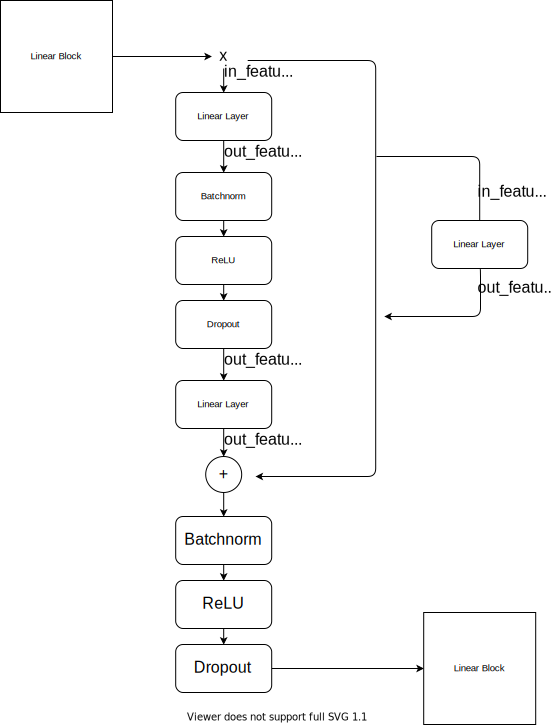
\includegraphics[width=0.7\textwidth]{mlp_architecture.png}
    \caption{Architecture of each Block in the Fully Connected Neural Network}
    \label{fig:linear-block}
\end{figure}
%%%

The structure of each so-called \texttt{Linear Block} is displayed in figure \ref{fig:linear-block}.
We now explain the reasoning behind including or excluding elements in this configuration.

\textbf{Linear Layer} \\
Each \texttt{Linear Block} is based on a four-element cycle that is repeated twice.
Each cycle starts with a Fully-Connected Layer containing the majority of trainable weights in the network.
The first linear layer determines the output dimension of this block, in our case mostly doubling or halving the number of input features.
Since both linear layers are immediately followed by a \texttt{Batchnorm} Layer, the additional \texttt{Bias} term is redundant and thus omitted.

\textbf{Batchnorm} \\
\texttt{Batchnorm} Layers often lead to a more well-behaved training process.
By means of first standardizing the activations within each minibatch and rescaling them afterwards, the network \emph{learns} a convenient magnitude of the activations.
This tends to be particularly effective for \emph{saturating} activation functions such as \texttt{sigmoid} or \texttt{tanh} activations, positive effects for training, however, have also been observed for the \texttt{ReLU} activation function, which is used in our design.
Of all individual components of the \texttt{Linear Block} structure, Batchnorm was the least important and provided only marginal benefits.

\textbf{ReLU} \\
Out of the numerous options for including nonlinearities into the network and thus expanding the function space that the network is able to learn, we settled for the default choice of the \emph{Rectified Linear Unit} activation.
While briefly experimenting with the related \texttt{Leaky ReLU} and \texttt{Exponential ReLU}, the differences were insignificant and could be easily attributed to other factors such as random weight initialization.

\textbf{Dropout} \\
The \texttt{Dropout} Layer at the end of each cycle turned out to be the single most impactful factor for the network's \emph{generalization} ability.
In fact, due to the different behaviour of dropout during training and inference, we could directly control the relative performance on training and validation set by varying the dropout probability $p$.

More specifically, the network overfitted drastically by setting $p$ to zero.
This actually provided the valuable insight that the current function class is flexible enough to model the task at hand properly.
Thus, there was no need to artificially expand the network size beyond the current quite compact architecture with roughly $280.000$ trainable parameters, saving computation time as a nice side-effect.

Figure \ref{fig:dropout} displays the shift in performance metrics on training and validation set when steadily increasing the dropout probability $p$.
While not beneficial for overall performance, dropout delivers a leverage to make the model perform much better on out-of-sample data compared to the dataset that it was actually trained on.

This behaviour can be explained by the \emph{ensemble} interpretation of dropout:
In each epoch, a different subset of neurons is excluded to contribute to training and thus a distinct subset model, nested in the full model, is responsible for the prediction output.
If the dropout probability is extremely high, these subset models are simply too different from each other and do \emph{not agree} on a common range of sensible prediction values.

In contrast, during inference (and possible deployment of the model), any randomness should be avoided and the network may use all of its neurons.
Although there is no influence on the model \emph{weights} in this stage, the model pools all subset models together and \emph{averages out} the diverging effects of each component, ultimately resulting in better performance metrics.

\textbf{Residual Connections} \\
One special feature of the \texttt{Linear Block} architecture in \ref{fig:linear-block} is the \emph{Residual Connection} adding the block input to the output of the second linear layer within each block.
This component was originally implemented having a fairly deep network in mind since \emph{Residual Blocks} introduced by the famous \texttt{ResNet} architecture are a very popular tool for stable gradient flow by preventing the issue of vanishing gradients.

As mentioned above the actual depth of the final model turned out to be limited.
Therefore we decided to enable inclusion and exclusion of skip-connections in the network by a \texttt{boolean} parameter allowing for easy comparisons between the model designs.
Although the residual component did not have a major impact on performance, it was slightly beneficial in most settings such that there was no reason to remove it from the architecture.

There are two aspects worth mentioning about the residual connection in figure \ref{fig:linear-block}:
%%%
\begin{enumerate}
    \item The addition of the input with the output of the second linear layer is performed \textbf{before} the final \texttt{Batchnorm} and \texttt{ReLU} layers of this block.
          This guarantees a nonnegative input in the expected range for the next \texttt{Linear Block} since the raw outputs of a fully connected layer are (in theory) unbounded.

    \item One caveat of the residual architecture is to ensure that at addition time all contributing terms share the same dimensions.
          In case of a fully connected layer dealing with two-dimensional tensors, this amounts to an equal number of features in the second dimension.
          As illustrated by the annotations in figure \ref{fig:linear-block}, this restriction requires an extra step if the number of input features is different from the number of output features in this particular block.
          In our case the dimnesions adjustment is performed by an additional linear layer exclusively for the block input $x$.
\end{enumerate}
%%%


\subsection{Further (Hyper)-Parameters}

\textbf{Optimizer and Weight Decay} \\
We used the popular \texttt{Adam} algorithm for training the Neural Network.
Compared to vanilla Gradient Descent (with optional momentum) the loss curves during the training process looked much smoother.
Moreover, while pure Gradient Descent slightly benefitted from an additonal weight penalty, neither the classical $L_2$ weight decay nor any other weight regularizer indicated improvements for training with Adam.

\textbf{Loss Function} \\
For the regression task of predicting the continuous price variable, we chose the standard continuously differentiable \emph{Mean Squared Error} loss function.
This come with the additional nice property that, under the assumption of a conditional normal distribution of the price with constant variance, i.e. $y_i \mid \mathbf{x}_i \sim \mathcal{N} \left(\mu_i, \sigma^2 \right)$, the model \emph{minimizing} the MSE-Loss simultaneously \emph{maximizes} the Gaussian Likelihood, providing a \emph{probabilistic} interpretation.

\textbf{Learning Rate} \\
Throughout training we kept the learning rate fixed at $0.01$.
Using a larger learning rate at early stages of training showed promising effects such that we experimented with different learning rate \emph{schedulers}, either decreasing the learning rate in fixed intervals linearly or exponentially, or decreasing the learning rate whenever the loss seems to stagnate for some given window.

However, the benefits of faster loss decay at the beginning of training were outweighed by too small learning rates at later stages in the training loop.
As a consequence, all schedulers resulted in stagnating loss much faster than training with a constant learning rate from start to end.

Moreover, since computation time was not too expensive due to the compact network size, we could make up for the slower initial progress that could be achieved with a scheduler by simply training the model for more epochs (while saving the model weights at the point of best performance on the validation set), which ultimately lead to a lower training and validation loss.


\newpage

\bibliography{bib}
\bibliographystyle{apalike}

\appendix

%%%
\begin{figure}[t]
    \centering
    \includegraphics[width=\textwidth]{dropout_performance.png}
    \caption{Impact of Dropout Probability on Training and Validation Performance}
    \label{fig:dropout}
\end{figure}
%%%



\end{document}